% SOURCE: edit-harness/results/frame_a/cells/cell_*_real_MIX_{A,B,C}_*.json + p2_llama-3.2-1b_real_MIX_C.json
% !TEX encoding = UTF-8 Unicode
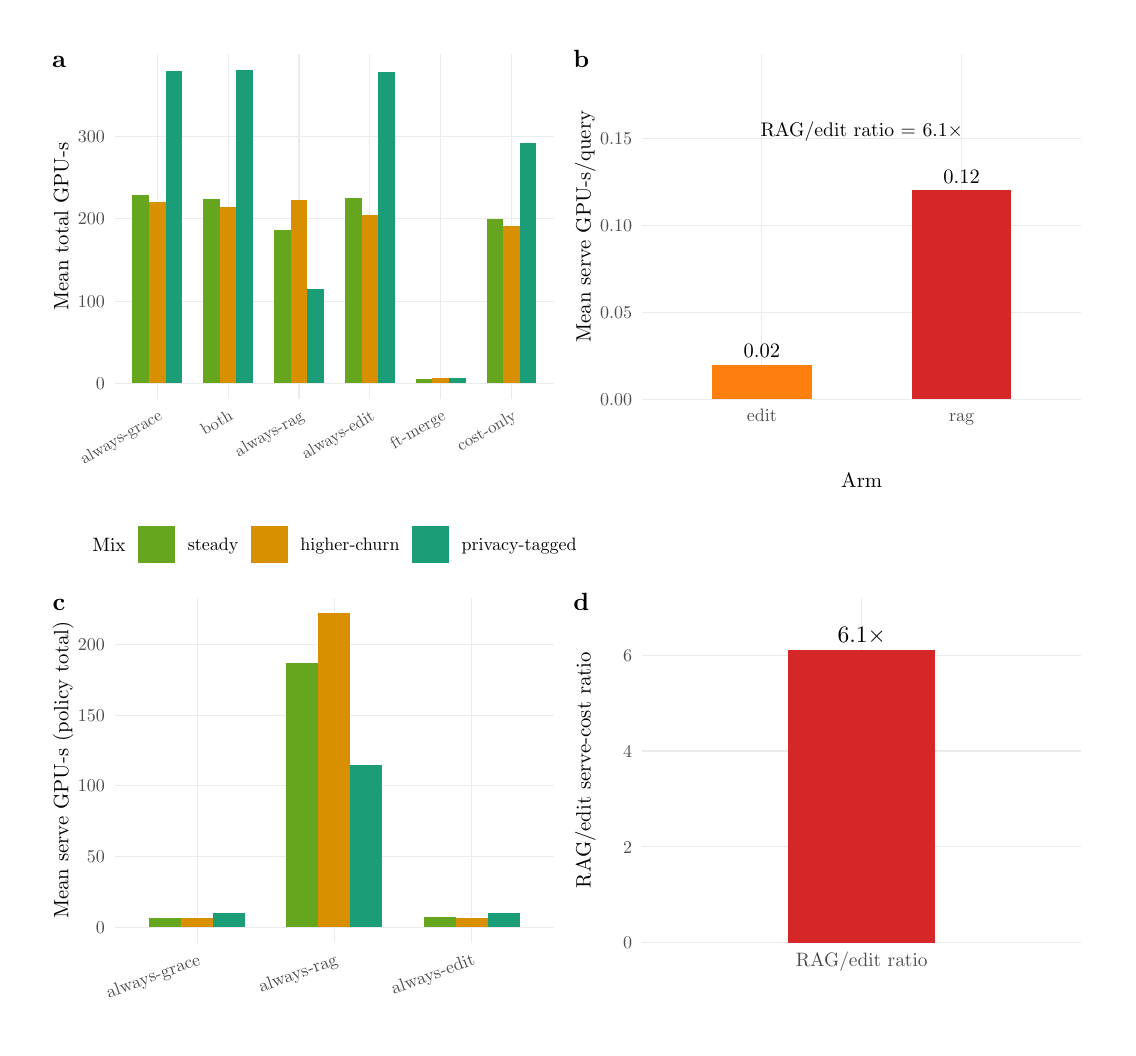
\begin{tikzpicture}[x=1pt,y=1pt]
\definecolor{fillColor}{RGB}{255,255,255}
\path[use as bounding box,fill=fillColor,fill opacity=0.00] (0,0) rectangle (390.26,361.35);
\begin{scope}
\path[clip] (  0.00,  0.00) rectangle (390.26,361.35);
\definecolor{drawColor}{RGB}{255,255,255}
\definecolor{fillColor}{RGB}{255,255,255}

\path[draw=drawColor,line width= 0.6pt,line join=round,line cap=round,fill=fillColor] (  0.00,  0.00) rectangle (390.26,361.35);
\end{scope}
\begin{scope}
\path[clip] (  5.50,159.41) rectangle (194.23,355.85);
\definecolor{fillColor}{RGB}{255,255,255}

\path[fill=fillColor] (  5.50,159.41) rectangle (194.23,355.85);
\end{scope}
\begin{scope}
\path[clip] (194.23,159.41) rectangle (384.76,355.85);
\definecolor{fillColor}{RGB}{255,255,255}

\path[fill=fillColor] (194.23,159.41) rectangle (384.76,355.85);
\end{scope}
\begin{scope}
\path[clip] (  5.50,  5.50) rectangle (194.23,159.41);
\definecolor{fillColor}{RGB}{255,255,255}

\path[fill=fillColor] (  5.50,  5.50) rectangle (194.23,159.41);
\end{scope}
\begin{scope}
\path[clip] (194.23,  5.50) rectangle (384.76,159.41);
\definecolor{fillColor}{RGB}{255,255,255}

\path[fill=fillColor] (194.23,  5.50) rectangle (384.76,159.41);
\end{scope}
\begin{scope}
\path[clip] ( 31.47,227.11) rectangle (190.23,351.85);
\definecolor{drawColor}{gray}{0.92}

\path[draw=drawColor,line width= 0.4pt,line join=round] ( 31.47,232.78) --
	(190.23,232.78);

\path[draw=drawColor,line width= 0.4pt,line join=round] ( 31.47,262.56) --
	(190.23,262.56);

\path[draw=drawColor,line width= 0.4pt,line join=round] ( 31.47,292.34) --
	(190.23,292.34);

\path[draw=drawColor,line width= 0.4pt,line join=round] ( 31.47,322.11) --
	(190.23,322.11);

\path[draw=drawColor,line width= 0.4pt,line join=round] ( 46.83,227.11) --
	( 46.83,351.85);

\path[draw=drawColor,line width= 0.4pt,line join=round] ( 72.44,227.11) --
	( 72.44,351.85);

\path[draw=drawColor,line width= 0.4pt,line join=round] ( 98.05,227.11) --
	( 98.05,351.85);

\path[draw=drawColor,line width= 0.4pt,line join=round] (123.65,227.11) --
	(123.65,351.85);

\path[draw=drawColor,line width= 0.4pt,line join=round] (149.26,227.11) --
	(149.26,351.85);

\path[draw=drawColor,line width= 0.4pt,line join=round] (174.86,227.11) --
	(174.86,351.85);
\definecolor{fillColor}{RGB}{102,166,31}

\path[fill=fillColor] ( 37.87,232.78) rectangle ( 43.85,300.98);

\path[fill=fillColor] ( 63.48,232.78) rectangle ( 69.45,299.51);

\path[fill=fillColor] ( 89.08,232.78) rectangle ( 95.06,288.34);

\path[fill=fillColor] (114.69,232.78) rectangle (120.66,299.91);

\path[fill=fillColor] (140.30,232.78) rectangle (146.27,234.54);

\path[fill=fillColor] (165.90,232.78) rectangle (171.88,292.24);
\definecolor{fillColor}{RGB}{216,144,0}

\path[fill=fillColor] ( 43.85,232.78) rectangle ( 49.82,298.29);

\path[fill=fillColor] ( 69.45,232.78) rectangle ( 75.43,296.61);

\path[fill=fillColor] ( 95.06,232.78) rectangle (101.03,298.91);

\path[fill=fillColor] (120.66,232.78) rectangle (126.64,293.78);

\path[fill=fillColor] (146.27,232.78) rectangle (152.24,234.76);

\path[fill=fillColor] (171.88,232.78) rectangle (177.85,289.81);
\definecolor{fillColor}{RGB}{27,158,119}

\path[fill=fillColor] ( 49.82,232.78) rectangle ( 55.80,345.52);

\path[fill=fillColor] ( 75.43,232.78) rectangle ( 81.40,346.18);

\path[fill=fillColor] (101.03,232.78) rectangle (107.01,266.87);

\path[fill=fillColor] (126.64,232.78) rectangle (132.61,345.31);

\path[fill=fillColor] (152.24,232.78) rectangle (158.22,234.69);

\path[fill=fillColor] (177.85,232.78) rectangle (183.83,319.76);
\end{scope}
\begin{scope}
\path[clip] (  0.00,  0.00) rectangle (390.26,361.35);
\definecolor{drawColor}{gray}{0.30}

\node[text=drawColor,anchor=base east,inner sep=0pt, outer sep=0pt, scale=  0.65] at ( 27.87,230.55) {0};

\node[text=drawColor,anchor=base east,inner sep=0pt, outer sep=0pt, scale=  0.65] at ( 27.87,260.32) {100};

\node[text=drawColor,anchor=base east,inner sep=0pt, outer sep=0pt, scale=  0.65] at ( 27.87,290.10) {200};

\node[text=drawColor,anchor=base east,inner sep=0pt, outer sep=0pt, scale=  0.65] at ( 27.87,319.87) {300};
\end{scope}
\begin{scope}
\path[clip] (  0.00,  0.00) rectangle (390.26,361.35);
\definecolor{drawColor}{gray}{0.30}

\node[text=drawColor,rotate= 30.00,anchor=base east,inner sep=0pt, outer sep=0pt, scale=  0.60] at ( 48.90,219.94) {always-grace};

\node[text=drawColor,rotate= 30.00,anchor=base east,inner sep=0pt, outer sep=0pt, scale=  0.60] at ( 74.51,219.94) {both};

\node[text=drawColor,rotate= 30.00,anchor=base east,inner sep=0pt, outer sep=0pt, scale=  0.60] at (100.11,219.94) {always-rag};

\node[text=drawColor,rotate= 30.00,anchor=base east,inner sep=0pt, outer sep=0pt, scale=  0.60] at (125.72,219.94) {always-edit};

\node[text=drawColor,rotate= 30.00,anchor=base east,inner sep=0pt, outer sep=0pt, scale=  0.60] at (151.32,219.94) {ft-merge};

\node[text=drawColor,rotate= 30.00,anchor=base east,inner sep=0pt, outer sep=0pt, scale=  0.60] at (176.93,219.94) {cost-only};
\end{scope}
\begin{scope}
\path[clip] (  0.00,  0.00) rectangle (390.26,361.35);
\definecolor{drawColor}{RGB}{0,0,0}

\node[text=drawColor,rotate= 90.00,anchor=base,inner sep=0pt, outer sep=0pt, scale=  0.75] at ( 14.67,289.48) {Mean total GPU-s};
\end{scope}
\begin{scope}
\path[clip] (  0.00,  0.00) rectangle (390.26,361.35);
\definecolor{drawColor}{RGB}{0,0,0}

\node[text=drawColor,anchor=base west,inner sep=0pt, outer sep=0pt, scale=  0.70] at ( 23.35,172.23) {Mix};
\end{scope}
\begin{scope}
\path[clip] (  0.00,  0.00) rectangle (390.26,361.35);
\definecolor{fillColor}{RGB}{102,166,31}

\path[fill=fillColor] ( 39.92,167.93) rectangle ( 53.34,181.35);
\end{scope}
\begin{scope}
\path[clip] (  0.00,  0.00) rectangle (390.26,361.35);
\definecolor{fillColor}{RGB}{216,144,0}

\path[fill=fillColor] ( 80.64,167.93) rectangle ( 94.06,181.35);
\end{scope}
\begin{scope}
\path[clip] (  0.00,  0.00) rectangle (390.26,361.35);
\definecolor{fillColor}{RGB}{27,158,119}

\path[fill=fillColor] (138.87,167.93) rectangle (152.29,181.35);
\end{scope}
\begin{scope}
\path[clip] (  0.00,  0.00) rectangle (390.26,361.35);
\definecolor{drawColor}{RGB}{0,0,0}

\node[text=drawColor,anchor=base west,inner sep=0pt, outer sep=0pt, scale=  0.65] at ( 57.86,172.40) {steady};
\end{scope}
\begin{scope}
\path[clip] (  0.00,  0.00) rectangle (390.26,361.35);
\definecolor{drawColor}{RGB}{0,0,0}

\node[text=drawColor,anchor=base west,inner sep=0pt, outer sep=0pt, scale=  0.65] at ( 98.58,172.40) {higher-churn};
\end{scope}
\begin{scope}
\path[clip] (  0.00,  0.00) rectangle (390.26,361.35);
\definecolor{drawColor}{RGB}{0,0,0}

\node[text=drawColor,anchor=base west,inner sep=0pt, outer sep=0pt, scale=  0.65] at (156.81,172.40) {privacy-tagged};
\end{scope}
\begin{scope}
\path[clip] (  0.00,  0.00) rectangle (390.26,361.35);
\definecolor{drawColor}{RGB}{0,0,0}

\node[text=drawColor,anchor=base,inner sep=0pt, outer sep=0pt, scale=  0.90] at ( 11.31,346.86) {\bfseries a};
\end{scope}
\begin{scope}
\path[clip] (222.00,227.11) rectangle (380.76,351.85);
\definecolor{drawColor}{gray}{0.92}

\path[draw=drawColor,line width= 0.4pt,line join=round] (222.00,227.11) --
	(380.76,227.11);

\path[draw=drawColor,line width= 0.4pt,line join=round] (222.00,258.55) --
	(380.76,258.55);

\path[draw=drawColor,line width= 0.4pt,line join=round] (222.00,289.99) --
	(380.76,289.99);

\path[draw=drawColor,line width= 0.4pt,line join=round] (222.00,321.42) --
	(380.76,321.42);

\path[draw=drawColor,line width= 0.4pt,line join=round] (265.30,227.11) --
	(265.30,351.85);

\path[draw=drawColor,line width= 0.4pt,line join=round] (337.46,227.11) --
	(337.46,351.85);
\definecolor{fillColor}{RGB}{255,127,14}

\path[fill=fillColor] (247.26,227.11) rectangle (283.34,239.49);
\definecolor{fillColor}{RGB}{214,39,40}

\path[fill=fillColor] (319.42,227.11) rectangle (355.50,302.61);
\definecolor{drawColor}{RGB}{0,0,0}

\node[text=drawColor,anchor=base,inner sep=0pt, outer sep=0pt, scale=  0.74] at (265.30,242.04) {0.02};

\node[text=drawColor,anchor=base,inner sep=0pt, outer sep=0pt, scale=  0.74] at (337.46,305.16) {0.12};

\node[text=drawColor,anchor=base,inner sep=0pt, outer sep=0pt, scale=  0.71] at (301.38,322.11) {RAG/edit ratio = 6.1$\times$};
\end{scope}
\begin{scope}
\path[clip] (  0.00,  0.00) rectangle (390.26,361.35);
\definecolor{drawColor}{gray}{0.30}

\node[text=drawColor,anchor=base east,inner sep=0pt, outer sep=0pt, scale=  0.65] at (218.40,224.88) {0.00};

\node[text=drawColor,anchor=base east,inner sep=0pt, outer sep=0pt, scale=  0.65] at (218.40,256.31) {0.05};

\node[text=drawColor,anchor=base east,inner sep=0pt, outer sep=0pt, scale=  0.65] at (218.40,287.75) {0.10};

\node[text=drawColor,anchor=base east,inner sep=0pt, outer sep=0pt, scale=  0.65] at (218.40,319.18) {0.15};
\end{scope}
\begin{scope}
\path[clip] (  0.00,  0.00) rectangle (390.26,361.35);
\definecolor{drawColor}{gray}{0.30}

\node[text=drawColor,anchor=base,inner sep=0pt, outer sep=0pt, scale=  0.65] at (265.30,219.04) {edit};

\node[text=drawColor,anchor=base,inner sep=0pt, outer sep=0pt, scale=  0.65] at (337.46,219.04) {rag};
\end{scope}
\begin{scope}
\path[clip] (  0.00,  0.00) rectangle (390.26,361.35);
\definecolor{drawColor}{RGB}{0,0,0}

\node[text=drawColor,anchor=base,inner sep=0pt, outer sep=0pt, scale=  0.75] at (301.38,195.32) {Arm};
\end{scope}
\begin{scope}
\path[clip] (  0.00,  0.00) rectangle (390.26,361.35);
\definecolor{drawColor}{RGB}{0,0,0}

\node[text=drawColor,rotate= 90.00,anchor=base,inner sep=0pt, outer sep=0pt, scale=  0.75] at (203.39,289.48) {Mean serve GPU-s/query};
\end{scope}
\begin{scope}
\path[clip] (  0.00,  0.00) rectangle (390.26,361.35);
\definecolor{drawColor}{RGB}{0,0,0}

\node[text=drawColor,anchor=base,inner sep=0pt, outer sep=0pt, scale=  0.90] at (200.05,346.86) {\bfseries b};
\end{scope}
\begin{scope}
\path[clip] ( 31.47, 30.67) rectangle (190.23,155.41);
\definecolor{drawColor}{gray}{0.92}

\path[draw=drawColor,line width= 0.4pt,line join=round] ( 31.47, 36.34) --
	(190.23, 36.34);

\path[draw=drawColor,line width= 0.4pt,line join=round] ( 31.47, 61.88) --
	(190.23, 61.88);

\path[draw=drawColor,line width= 0.4pt,line join=round] ( 31.47, 87.41) --
	(190.23, 87.41);

\path[draw=drawColor,line width= 0.4pt,line join=round] ( 31.47,112.94) --
	(190.23,112.94);

\path[draw=drawColor,line width= 0.4pt,line join=round] ( 31.47,138.47) --
	(190.23,138.47);

\path[draw=drawColor,line width= 0.4pt,line join=round] ( 61.24, 30.67) --
	( 61.24,155.41);

\path[draw=drawColor,line width= 0.4pt,line join=round] (110.85, 30.67) --
	(110.85,155.41);

\path[draw=drawColor,line width= 0.4pt,line join=round] (160.46, 30.67) --
	(160.46,155.41);
\definecolor{fillColor}{RGB}{102,166,31}

\path[fill=fillColor] ( 43.87, 36.34) rectangle ( 55.45, 39.71);

\path[fill=fillColor] ( 93.48, 36.34) rectangle (105.06,131.62);

\path[fill=fillColor] (143.10, 36.34) rectangle (154.67, 39.90);
\definecolor{fillColor}{RGB}{216,144,0}

\path[fill=fillColor] ( 55.45, 36.34) rectangle ( 67.03, 39.59);

\path[fill=fillColor] (105.06, 36.34) rectangle (116.64,149.74);

\path[fill=fillColor] (154.67, 36.34) rectangle (166.25, 39.80);
\definecolor{fillColor}{RGB}{27,158,119}

\path[fill=fillColor] ( 67.03, 36.34) rectangle ( 78.60, 41.54);

\path[fill=fillColor] (116.64, 36.34) rectangle (128.21, 94.79);

\path[fill=fillColor] (166.25, 36.34) rectangle (177.82, 41.35);
\end{scope}
\begin{scope}
\path[clip] (  0.00,  0.00) rectangle (390.26,361.35);
\definecolor{drawColor}{gray}{0.30}

\node[text=drawColor,anchor=base east,inner sep=0pt, outer sep=0pt, scale=  0.65] at ( 27.87, 34.11) {0};

\node[text=drawColor,anchor=base east,inner sep=0pt, outer sep=0pt, scale=  0.65] at ( 27.87, 59.64) {50};

\node[text=drawColor,anchor=base east,inner sep=0pt, outer sep=0pt, scale=  0.65] at ( 27.87, 85.17) {100};

\node[text=drawColor,anchor=base east,inner sep=0pt, outer sep=0pt, scale=  0.65] at ( 27.87,110.70) {150};

\node[text=drawColor,anchor=base east,inner sep=0pt, outer sep=0pt, scale=  0.65] at ( 27.87,136.24) {200};
\end{scope}
\begin{scope}
\path[clip] (  0.00,  0.00) rectangle (390.26,361.35);
\definecolor{drawColor}{gray}{0.30}

\node[text=drawColor,rotate= 20.00,anchor=base east,inner sep=0pt, outer sep=0pt, scale=  0.65] at ( 62.77, 22.87) {always-grace};

\node[text=drawColor,rotate= 20.00,anchor=base east,inner sep=0pt, outer sep=0pt, scale=  0.65] at (112.38, 22.87) {always-rag};

\node[text=drawColor,rotate= 20.00,anchor=base east,inner sep=0pt, outer sep=0pt, scale=  0.65] at (161.99, 22.87) {always-edit};
\end{scope}
\begin{scope}
\path[clip] (  0.00,  0.00) rectangle (390.26,361.35);
\definecolor{drawColor}{RGB}{0,0,0}

\node[text=drawColor,rotate= 90.00,anchor=base,inner sep=0pt, outer sep=0pt, scale=  0.75] at ( 14.67, 93.04) {Mean serve GPU-s (policy total)};
\end{scope}
\begin{scope}
\path[clip] (  0.00,  0.00) rectangle (390.26,361.35);
\definecolor{drawColor}{RGB}{0,0,0}

\node[text=drawColor,anchor=base,inner sep=0pt, outer sep=0pt, scale=  0.90] at ( 11.31,150.85) {\bfseries c};
\end{scope}
\begin{scope}
\path[clip] (222.00, 30.67) rectangle (380.76,155.41);
\definecolor{drawColor}{gray}{0.92}

\path[draw=drawColor,line width= 0.4pt,line join=round] (222.00, 30.67) --
	(380.76, 30.67);

\path[draw=drawColor,line width= 0.4pt,line join=round] (222.00, 65.32) --
	(380.76, 65.32);

\path[draw=drawColor,line width= 0.4pt,line join=round] (222.00, 99.97) --
	(380.76, 99.97);

\path[draw=drawColor,line width= 0.4pt,line join=round] (222.00,134.62) --
	(380.76,134.62);

\path[draw=drawColor,line width= 0.4pt,line join=round] (301.38, 30.67) --
	(301.38,155.41);
\definecolor{fillColor}{RGB}{214,39,40}

\path[fill=fillColor] (274.92, 30.67) rectangle (327.84,136.38);
\definecolor{drawColor}{RGB}{0,0,0}

\node[text=drawColor,anchor=base,inner sep=0pt, outer sep=0pt, scale=  0.85] at (301.38,139.32) {6.1$\times$};
\end{scope}
\begin{scope}
\path[clip] (  0.00,  0.00) rectangle (390.26,361.35);
\definecolor{drawColor}{gray}{0.30}

\node[text=drawColor,anchor=base east,inner sep=0pt, outer sep=0pt, scale=  0.65] at (218.40, 28.44) {0};

\node[text=drawColor,anchor=base east,inner sep=0pt, outer sep=0pt, scale=  0.65] at (218.40, 63.09) {2};

\node[text=drawColor,anchor=base east,inner sep=0pt, outer sep=0pt, scale=  0.65] at (218.40, 97.73) {4};

\node[text=drawColor,anchor=base east,inner sep=0pt, outer sep=0pt, scale=  0.65] at (218.40,132.38) {6};
\end{scope}
\begin{scope}
\path[clip] (  0.00,  0.00) rectangle (390.26,361.35);
\definecolor{drawColor}{gray}{0.30}

\node[text=drawColor,anchor=base,inner sep=0pt, outer sep=0pt, scale=  0.70] at (301.38, 22.25) {RAG/edit ratio};
\end{scope}
\begin{scope}
\path[clip] (  0.00,  0.00) rectangle (390.26,361.35);
\definecolor{drawColor}{RGB}{0,0,0}

\node[text=drawColor,rotate= 90.00,anchor=base,inner sep=0pt, outer sep=0pt, scale=  0.75] at (203.39, 93.04) {RAG/edit serve-cost ratio};
\end{scope}
\begin{scope}
\path[clip] (  0.00,  0.00) rectangle (390.26,361.35);
\definecolor{drawColor}{RGB}{0,0,0}

\node[text=drawColor,anchor=base,inner sep=0pt, outer sep=0pt, scale=  0.90] at (200.05,150.85) {\bfseries d};
\end{scope}
\end{tikzpicture}
